\begin{figure}[!h]
  \centering
  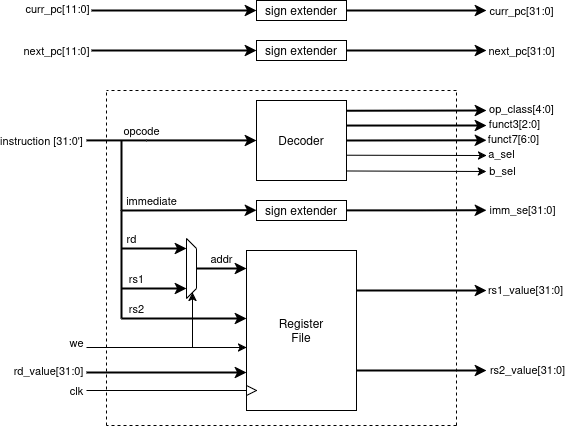
\includegraphics[scale=0.4]{ID_BD.png}
  \caption{A block diagram for the instruction decoding stage}
  \label{fig:ID_BD}
\end{figure}

\section{Instruction formats}
After an instruction is returned from the fetching stage, it must be decoded in order to select the right action that has to be performed in the next step of the datapath. The RISC-V ISA provides instructions for register to operate with other registers, constants, with the data memory or the PC itself.
In the base ISA, there are four core instruction formats:
\begin{itemize}
\item \textbf{R-type}: Register to register instructions. These instructions are expected to use two registers as sorce for data to be elaborated and then store the result of the operation in a destination register. This instruction has to select the two sources as operands for the next stage to treat them as such, hence two boolean outputs \emph{a\_sel} and \emph{b\_sel} will be pulled high to indicate that the registers pointed by the values of rs1 (bits 19 down to 15) and rs2 (bits 24 down to 20) are used as operands.
\item \textbf{I-type}: Immediate instructions. The value stored in rs1 (bits 19 to 15) and an immediate value (bits 31 to 20) make the operands of the operation to be executed. \emph{a\_sel} has to be set high while \emph{b\_sel} is set to low.
\item \textbf{S-type}: For store operations, where the content of the register rs2 is stored inside the memory address in the data memory pointed by rs1, possibly summed to an immediate value (little endian encoded, bits 31 to 25 for the 7 most significant bits and bits 11 to 7 for the least significant ones). In this case \emph{a\_sel} is set to high while \emph{b\_sel} stays low in order for the ALU to sum rs2 and the immediate value.
\item \textbf{U-type}: Loading immediates inside a register, like for example the the LUI (Load Upper Immediate) instruction. In this case just \emph{b\_sel} is needed to be low while the value of the other output is not negligible.
\end{itemize}
These instructions share the same positions for the operands and the destination registers, which simplifies the structure of the code (Figure \ref{fig:base_form}).
\begin{figure}[h!]
  \centering
  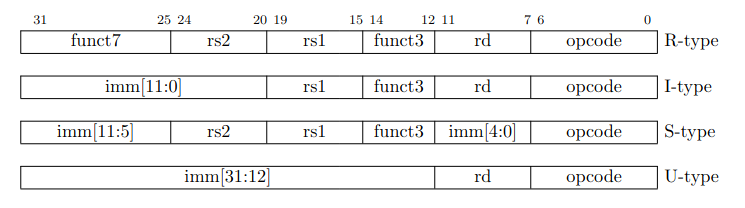
\includegraphics[scale=0.6]{base_isa.png}
  \caption{Base instruction format \cite{waterman2016riscv}}
  \label{fig:base_form}
\end{figure}
Instructions that operate with the PC and conditional instructions such as branches share similar structure with respectively U-type and S-type instructions, in the ISA they are defined as:
\begin{itemize}
  \item \textbf{B-type} or SB-type: Just as in store operations, the rs1 and rs2 addresses are coded in the same position, with the difference that the immediate value has its bits coded in different positions (imm[12] on bit 31, imm[11] on bit 7, imm[10:5] from bit 30 to 25, imm[4:1] from bit 11 to 8). For this type of operation there is no need to change \emph{a\_sel} and \emph{b\_sel}, since, as it will be shown later, the logic unit just operates between registers.
  \item \textbf{J-type} or UJ-type: Jump operations load sums an immediate to the PC and stores the next instruction's PC value. These are coded just as unsigned operations, with the difference being the immediate's bits having different positions (imm[20] on position 31, imm[19:12] from position 19 to 12, imm[11] on bit 20 and imm[10:1] from position 30 to 21).
\end{itemize}
With these definitions, the base ISA extends to this:

\begin{figure}[h!]
  \centering
  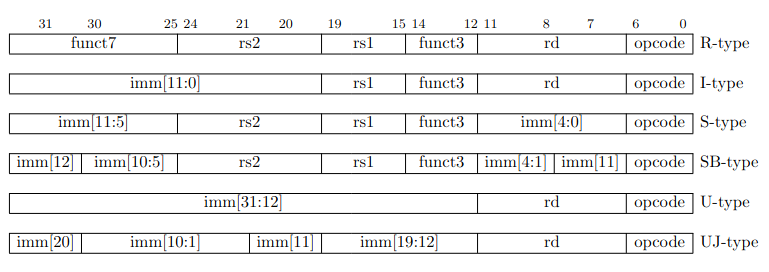
\includegraphics[scale=0.58]{base_isa_2.png}
  \caption{Full 32-bit instruction format \cite{waterman2016riscv}}
  \label{fig:full_form}
\end{figure}
Knowing that the next block can be programmed to use certain parts of the instruction in a certain way, the VHDL code for the ID architecture can be simplified by giving out all the sections of the instruction and letting the Instruction Execute select what specific parts of it are needed.

\section{Decoding}
\subsection{Reading opcodes for operand selection}
The encoding type of an instruction is not sufficient to detect what operation is actually performed. For example, \emph{LW} and \emph{ADDI} are both I-type instructions but the latter has its result written somewhere in the Register File instead of the Data Memory.
For this reason it is necessary to assess some information segments inside the instruction itself. By looking at Figure \ref{fig:full_form} it is noticeable that there are at most three elements that are descriptive of the content of the instruction and its behavior:
\begin{itemize}
  \item \textbf{opcode}: Unique and present in every instruction, composed by the first 7 bits (starting from the LSB, considering a Little Endian encoding).
  \item \textbf{funct3}: Present in all instructions but U and J -types, made by bit 12 up to 14, necessary for the ALU to select the arithmetic or logic operation to be executed.
  \item \textbf{funct7}: Only for R-type instructions, in the RV32I ISA only one of the seven bits is used.
\end{itemize}
It's obvious that \emph{funct3} and \emph{funct7} do not give information about the identity of the instruction, it is the \emph{opcode} that differentiates the operation and therefore the one that has to be taken into account. The Instruction Set manual [described by Waterman et al. (2016) \cite{waterman2016riscv} page 53 Table 9.1] gives the general opcode map that can help to discriminate instructions: 

\begin{figure}[h!]
  \centering
  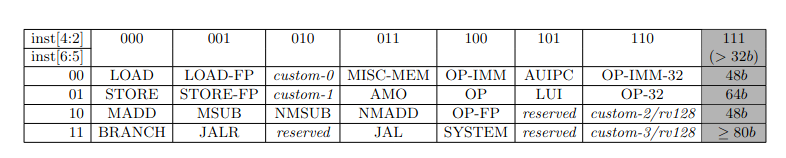
\includegraphics[scale=0.55]{opcodes.png}
  \caption{RISC-V base opcode map \cite{waterman2016riscv}} 
\end{figure}
In a non-superscalar design that does not take into account multiplications, floating-point operations, just implementing \textbf{LOAD}, \textbf{STORE}, \textbf{BRANCH}, \textbf{JALR}, \textbf{JAL}, \textbf{OP} and \textbf{OP-IMM} is sufficient.
The opcode map gives the idea that a decoder can be described with a nested case statement, with an external case structure driven by the last two bits of the opcode, from which is possible to extrapolate what are the operands to be passed to the ALU or Logic Unit, being it the PC, two registers or an immediate and a register.  

\subsection{Classification for the Write Back}
The last and most delicate problem that arises when decoding instructions is that they operate in different ways even if they share the same encoding type, for example, ADDI will write the result of the arithmetic operation in a destination register, while LW will have the destination register be a memory location pointed by the result of another arithmetic operation. Also, the interaction with the Program counter is different even between same-type instructions, hence there is the additional requirement to define in advance a classification method in advance so that the Write Back stage can select what can has to be passed to the Register File and select the next value for the Program Counter.
There are three possible cases in which the Write Back accesses the register file:
\begin{itemize}
  \item Jump Instructions (since they write back the return address)
  \item Load Instructions
  \item Arithmetic and logic operations
\end{itemize}
Also, the PC can have a new value loaded if, during a branch intruction, the Logic Unit returns a logic high, or during a jump instruction. Otherwise, PC+4 is always returned as next value.
The ID can encode these informations for the next stages as a 5 bit vector, with a one-hot encoding for Arithmetic-Logic Operations, Jump, Load and Store, since store operations can be added as an additional bit that can be used as a write-enable for the Data Memory.

\section{Final concept for the ID and simulation}
The finalized concept of the Instruction decode, which follows the block diagram at Figure \ref{fig:ID_BD}, introduces the Register File and a specialized block for decoding, taking as inputs all the IF's outputs (including {pc\_out} and {next\_pc} for sign extension).

\begin{minted}[fontsize=\footnotesize]{vhdl}
entity instr_decode is
  Port (
    clk         : in std_logic;
    instr       : in std_logic_vector(31 downto 0);
    next_pc     : in std_logic_vector(11 downto 0);
    curr_pc     : in std_logic_vector(11 downto 0);
    
    -- Inputs from mem writeback
    
    rd_write_en : in std_logic;
    rd_value    : in std_logic_vector(31 downto 0);
    
    -- sign-extended pc info
    
    next_pc_ze  : out std_logic_vector(31 downto 0);
    curr_pc_ze  : out std_logic_vector(31 downto 0);
    
    -- Decoded instruction informations
    
    op_class    : out std_logic_vector(4 downto 0);
    funct3      : out std_logic_vector(2 downto 0);
    funct7      : out std_logic_vector(6 downto 0);
    a_sel       : out std_logic;
    b_sel       : out std_logic;
    cond_opcode : out std_logic_vector(2 downto 0);
    
    -- Data to be elaborated
    
    rs1         : out std_logic_vector(31 downto 0);
    rs2         : out std_logic_vector(31 downto 0);
    imm_se      : out signed(31 downto 0)
  );
end instr_decode;

architecture Structural of instr_decode is
  signal rd_rs1_mux       : std_logic_vector(4 downto 0) := (others => '0');
  signal next_pc_ze_reg   : std_logic_vector(31 downto 0) := (others => '0');
  signal curr_pc_ze_reg   : std_logic_vector(31 downto 0) := (others => '0');
      
  -- components declarations
begin
  reg : register_file
  port map(
    clk         => clk,
    we          => rd_write_en,
    d           => rd_value,
    a           => rd_rs1_mux,
    dpra        => instr(24 downto 20),
    qspo        => rs1,
    qdpo        => rs2
  );
  
  dec : decoder
  port map(
    clk         => clk,
    instr       => instr,
    op_class    => op_class,
    funct3      => funct3,
    funct7      => funct7,
    a_sel       => a_sel,
    b_sel       => b_sel,
    cond_opcode => cond_opcode,
    imm_se      => imm_se
  );
    
  process(clk)
  begin
    if rising_edge(clk) then
      next_pc_ze_reg       <= std_logic_vector(resize(unsigned(next_pc), next_pc_ze_reg'length));
      curr_pc_ze_reg       <= std_logic_vector(resize(unsigned(curr_pc), next_pc_ze_reg'length));
    end if;
  end process;
  
  rd_rs1_mux  <= instr(11 downto 7) when rd_write_en = '1' else instr(19 downto 15);
  next_pc_ze  <= next_pc_ze_reg;
  curr_pc_ze  <= curr_pc_ze_reg;
end Structural;
\end{minted}

As it was done for the Instruction Memory, the Register File was added to the project through the Distributed Memory Generator IP, declared as a dual port RAM with 32 32-bit registers, hence with 5 address bits. The most complex part of this stage, the decoder, is implemented as two nested case statements, with the outer statement using the two most significant bits of the opcode. A snippet is provided down below for the concept used for decoding LOAD type instructions (opcode "00000"):

\begin{minted}[fontsize=\footnotesize]{vhdl}
process(clk)
begin
  if rising_edge(clk) then
    case instr(6 downto 5) is
      when "00" =>
        case instr(4 downto 2) is 
          when "000"  =>              -- LOAD [I-type]
            op_class_reg    <=  "00010";
            imm_se_reg      <=  resize(signed(instr(31 downto 20)), imm_se_reg'length); -- Sign extension 
            a_sel_reg       <=  '1'; -- Select register as first operand 
            b_sel_reg       <=  '0'; -- Select immediate as second operand
            alu_opcode_reg  <= "000"; -- Select add
            cond_opcode_reg <= "000";
          when "100"  =>              -- OP-IMM [I-type]
            op_class_reg    <=  "00001";
            imm_se_reg      <=  resize(signed(instr(31 downto 20)), imm_se_reg'length);
            a_sel_reg       <=  '1';
            b_sel_reg       <=  '0';
            alu_opcode_reg  <= instr(14 downto 12);
            cond_opcode_reg <= instr(14 downto 12);    
          when "101"  => 
            -- etc.
\end{minted}

By using the same testbench as for the IF and istantiating the ID, by routing the selected instruction and the PC's values, the code is expected to fetch the instruction 0x00000293 (\emph{addi x5 x0 0}, i.e. $x5 = x0 + 0$), decode it and classify it as an operation with an immediate as second operand, hence with \emph{a{\_}sel}=1, \emph{b{\_}sel}=0 and \emph{op{\_}class}=00010:

\begin{figure}[h!]
  \centering
  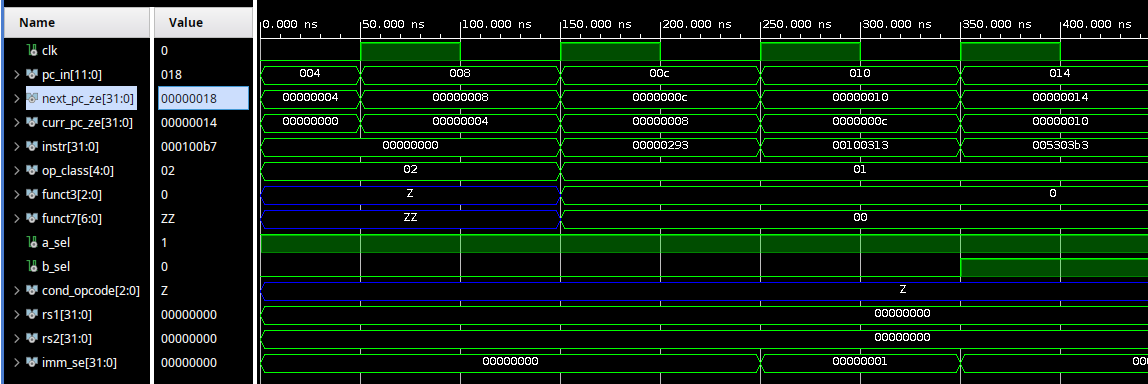
\includegraphics[scale=0.37]{ID_sim.png}
\end{figure}


\let\cleardoublepage\clearpage